\documentclass{standalone}
\usepackage{tikz}
\usepackage{ctex,siunitx}
\setCJKmainfont{Noto Serif CJK SC}
\usepackage{tkz-euclide}
\usepackage{amsmath}
\usetikzlibrary{patterns, calc,3d}
\usetikzlibrary {decorations.pathmorphing,decorations.pathreplacing,decorations.shapes,}
\tikzset{label style/.append style={font=\small}}
\begin{document}
\small
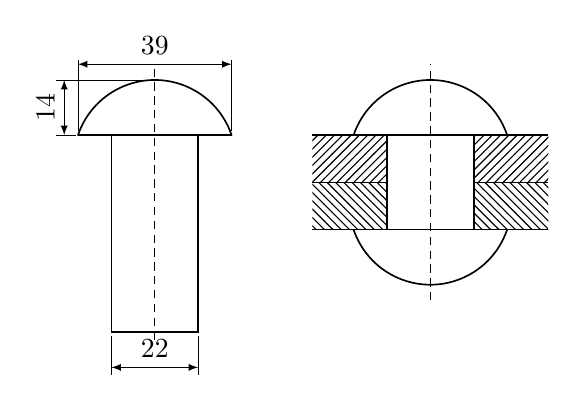
\begin{tikzpicture}[>=latex,scale=0.5]
  \begin{scope}
    \tkzDefPoints{-1.95/0/A,1.95/0/B,0/1.4/C,1.1/0/D,-1.1/-5.0/E}
    \tkzDefTriangleCenter(A,B,C)\tkzGetPoint{O1}
    \draw[semithick](D)rectangle(E);
    \tkzDrawArc[semithick](O1,B)(A)
    \tkzDrawSegments[semithick](A,B)
    \draw[densely dashed](0,-5.2)--(0,1.7);
    \draw[very thin](0,1.4)--(-2.5,1.4)(-2,0)--(-2.5,0)(-1.95,0.1)--(-1.95,1.9)(1.95,0.1)--(1.95,1.9)(-1.1,-5.1)--(-1.1,-6.1)(1.1,-5.1)--(1.1,-6.1);
    \draw[very thin,<->](-2.3,0)--(-2.3,1.4)node[midway,sloped,above]{14};
    \draw[very thin,<->](-1.95,1.8)--(1.95,1.8)node[midway,sloped,above]{39};
    \draw[very thin,<->](-1.1,-5.9)--(1.1,-5.9)node[midway,sloped,above]{22};
  \end{scope}
  \begin{scope}[xshift=7cm,yshift=-1.2cm]
    \tkzDefPoints{-1.95/1.2/A,1.95/1.2/B,0/2.6/C,1.1/1.2/D,-1.1/-1.2/E,-1.95/-1.2/A',1.95/-1.2/B',0/-2.6/C'}
    \tkzDefTriangleCenter(A,B,C)\tkzGetPoint{O1}
    \tkzDefTriangleCenter(A',B',C')\tkzGetPoint{O2}
    \draw[semithick](D)rectangle(E);
    \tkzDrawArc[semithick](O1,B)(A)
    \tkzDrawArc[semithick](O2,A')(B')
    \tkzDrawSegments[semithick](A,B A',B')
    \draw[densely dashed](0,-3.0)--(0,3.0);
    \draw[semithick,pattern=north east lines](-3,1.2)--(-1.1,1.2)--(-1.1,0)--(-3,0)(3,1.2)--(1.1,1.2)--(1.1,0)--(3,0);
    \draw[semithick,pattern=north west lines](-3,-1.2)--(-1.1,-1.2)--(-1.1,0)--(-3,0)(3,-1.2)--(1.1,-1.2)--(1.1,0)--(3,0);
  \end{scope}
\end{tikzpicture}
\end{document}